% Compile with:  tectonic --keep-logs paper.tex
% The Lean code in boxes is read from snip/*.lean, written by extract.py from snippets.txt.
\documentclass[11pt,a4paper]{article}

\usepackage{fontspec}
\usepackage[a4paper,margin=2.5cm]{geometry}
\usepackage{amsmath,amssymb,amsthm}
\usepackage{booktabs}
\usepackage{enumitem}
\usepackage{xcolor}
\usepackage{fvextra}
\usepackage{newunicodechar}
\usepackage{graphicx}
\usepackage{tikz}
\usetikzlibrary{shapes.geometric,calc,arrows.meta,decorations.markings}
\usepackage{caption}
\usepackage{float}
\PassOptionsToPackage{hyphens}{url}
\usepackage[hidelinks]{hyperref}

% ---- Fonts: a monospace font with the Unicode glyphs of the Lean sources -------------------
\IfFontExistsTF{Menlo}{\setmonofont{Menlo}[Scale=0.84]}{%
  \IfFontExistsTF{DejaVu Sans Mono}{\setmonofont{DejaVu Sans Mono}[Scale=0.84]}{}}
\IfFontExistsTF{STIX Two Math}{\newfontfamily\fallbackfont{STIX Two Math}[Scale=0.9]}{%
  \newfontfamily\fallbackfont{Latin Modern Math}}
% Characters of the Lean sources that the monospace font (Menlo) lacks: the subscript letters of
% `::ₘ`, `Sⁱₙ`, `xₖ`, and the script `ℓ`. Each is set in a box of the width of one monospace
% character, so that the columns of the listings stay aligned.
%
% Among the installed fonts only the macOS system font has the subscript letters. When it is
% there the real character is typeset (and can be searched and copied in the PDF). Elsewhere a
% lowered small letter is drawn instead.
\newcommand{\fbch}[1]{\makebox[0.602em][c]{\fallbackfont #1}}
\newcommand{\subdrawn}[1]{\makebox[0.602em][c]{\raisebox{-0.38ex}{\scalebox{0.7}{#1}}}}
\newif\ifsubfont
\IfFileExists{/System/Library/Fonts/SFNS.ttf}{\subfonttrue
  \newfontfamily\subfont{SFNS.ttf}[Path=/System/Library/Fonts/,Scale=0.95]}{\subfontfalse}
\newcommand{\subch}[2]{\ifsubfont\makebox[0.602em][c]{\subfont #1}\else\subdrawn{#2}\fi}
\newunicodechar{ₘ}{\subch{ₘ}{m}}
\newunicodechar{ₖ}{\subch{ₖ}{k}}
\newunicodechar{ₙ}{\subch{ₙ}{n}}
\newunicodechar{ℓ}{\fbch{ℓ}}


% ---- Notes to the author -------------------------------------------------------------------
\newcommand{\todo}[1]{\textcolor{red}{\textsf{\small[TODO: #1]}}}

% ---- Lean code, quoted from the repository --------------------------------------------------
\definecolor{codeframe}{gray}{0.70}
\newcommand{\lean}[1]{%
  \VerbatimInput[frame=single,rulecolor=\color{codeframe},framesep=1.6mm,breaklines=true,
    breakanywhere=false,breaksymbolleft={},samepage=true,fontsize=\fontsize{7.4}{9.0}\selectfont]{snip/#1.lean}}
\let\origus\_
\ExplSyntaxOn
\NewDocumentCommand{\cod}{m}{
  \group_begin:
  \tl_set:Nn \l_tmpa_tl {#1}
  \regex_replace_all:nnN { ([\.\/]) } { \1\c{allowbreak} } \l_tmpa_tl
  \ttfamily \cs_set:Npn \_ { \origus \allowbreak } \l_tmpa_tl
  \group_end:
}
\ExplSyntaxOff

% ---- Drawings of nets -----------------------------------------------------------------------
\tikzset{
  tri/.style={regular polygon,regular polygon sides=3,draw,line width=0.6pt,
    minimum size=11mm,inner sep=0pt},
  isdup/.style={fill=black!20},
  eracell/.style={circle,draw,line width=0.6pt,minimum size=5.6mm,inner sep=0pt,
    font=\fontsize{6}{6}\selectfont},
  wire/.style={line width=0.6pt},
  port/.style={font=\scriptsize\itshape,inner sep=1.2pt,text height=1.3ex,text depth=0.4ex},
  idx/.style={font=\fontsize{5.5}{5.5}\selectfont\sffamily,text=black!80,inner sep=0.6pt},
  boxtree/.style={draw,line width=0.6pt,minimum width=6mm,minimum height=4.5mm,inner sep=1pt,
    font=\scriptsize\itshape},
  becomes/.style={-{Stealth[length=2mm]},line width=0.6pt},
  nm/.style={circle,fill=black,inner sep=1.1pt},
}
% \cellD[style]{name}{position}{label}: principal port at the bottom; auxiliary port 0 on the left.
\newcommand{\cellD}[4][]{%
  \node[tri,shape border rotate=180,#1] (#2) at (#3) {};
  \node[font=\fontsize{6}{6}\selectfont] at ($(#2.center)+(0,0.07)$) {#4};
  \coordinate (#2-p) at (#2.corner 1);
  \coordinate (#2-0) at ($(#2.corner 3)!0.24!(#2.corner 2)$);
  \coordinate (#2-1) at ($(#2.corner 3)!0.76!(#2.corner 2)$);
  \node[idx,anchor=south east] at (#2-0) {0};
  \node[idx,anchor=south west] at (#2-1) {1};}
% \cellU[style]{name}{position}{label}: principal port at the top. It is the same cell turned by
% 180 degrees (Lafont, page 71), so auxiliary port 0 is on the RIGHT.
\newcommand{\cellU}[4][]{%
  \node[tri,#1] (#2) at (#3) {};
  \node[font=\fontsize{6}{6}\selectfont] at ($(#2.center)+(0,-0.07)$) {#4};
  \coordinate (#2-p) at (#2.corner 1);
  \coordinate (#2-0) at ($(#2.corner 2)!0.76!(#2.corner 3)$);
  \coordinate (#2-1) at ($(#2.corner 2)!0.24!(#2.corner 3)$);
  \node[idx,anchor=north west] at (#2-0) {0};
  \node[idx,anchor=north east] at (#2-1) {1};}
% A cell with one auxiliary port.
\newcommand{\cellOneU}[3]{%
  \node[tri] (#1) at (#2) {};
  \node[font=\fontsize{6}{6}\selectfont] at ($(#1.center)+(0,-0.07)$) {#3};
  \coordinate (#1-p) at (#1.corner 1);
  \coordinate (#1-0) at ($(#1.corner 2)!0.5!(#1.corner 3)$);}

% ---- Theorem-like environments ---------------------------------------------------------------
\newtheorem*{lafont}{Theorem 1 (Lafont)}

\newcommand{\Equiv}{\cod{Equiv}}
\newcommand{\pp}[1]{\cite[#1]{lafont1997}}

\setlist{itemsep=0.15em,topsep=0.3em}
\emergencystretch=3em
\captionsetup{font=small,labelfont=bf}

\title{A Machine-Checked Proof of the Universality of Interaction Combinators}

\author{Lorenzo Battistela\\[0.3em]\small Independent researcher}

\date{Draft of 20 November 2026}

\begin{document}
\maketitle
\nocite{lafont1997}

\begin{abstract}
\noindent
Lafont's interaction combinators are a graph-rewriting system with three symbols and six rules.
Their central property is universality: every interaction system can be translated into the
combinators in a way that preserves reduction. The published proof is drawn as pictures, and its
final step, that the general translation is compatible with reduction, is left to the reader. We
present a complete machine-checked proof of this theorem in Lean~4, including that step. Nets
are represented as text, as multisets of equations between trees, and we prove that this
representation agrees with nets as graphs, for the objects and for reduction, in both
directions. We prove the symmetric decomposition of the rule of a symbol with itself, which the
original proof derives from a canonical decomposition that it does not define. We also state
the theorem with the decomposition of the rules given as data, in which case the translation is
a computable function. The proofs were written by a swarm of autonomous language-model agents
that planned their own work, proved, and reviewed one another, against definitions and target
statements fixed and reviewed by the author.
\end{abstract}

%=================================================================================================
\section{Introduction}
\label{sec:intro}

Interaction nets were introduced by Lafont~\cite{lafont1990} as a model of computation in which
a program is a graph of \emph{cells} and computing is rewriting pairs of cells joined by their
principal ports. Rewriting is local and strongly confluent, so the order in which the pairs are
rewritten changes neither the result nor the number of steps. In \emph{Interaction
Combinators}~\cite{lafont1997} Lafont gave a system with three symbols, the constructor
$\gamma$, the duplicator $\delta$ and the eraser $\varepsilon$, and six rules
(Fig.~\ref{fig:rules}), and proved:

\begin{lafont}
Any interaction system can be translated into the system of interaction combinators.
\end{lafont}

A translation replaces each cell by a fixed net of combinators with the same ports, in such a
way that every reduction step of the source is simulated by a bounded number of steps of the
target (at least one, when the translation is \emph{strict}). This is a stronger notion of
universality than the ability to encode a Turing machine: it preserves the complexity and the
degree of parallelism of computations, and Lafont notes that a universal Turing machine, seen
as an interaction system, is not universal in this sense~\pp{p.~70}. By the theorem, three
symbols suffice as a target for compiling interaction nets. A symmetric variant of the
combinators, to which the theorem does not apply directly (Section~\ref{sec:limits}), is the
basis of practical evaluators such as HVM~\cite{hvm2}.

The published proof occupies Section~2 of~\cite{lafont1997} (pages 81 to 90) and consists
mostly of figures. A restricted case, recursion-free systems, is treated first, with a figure
(Fig.~7) that shows the translations of two cells reducing to the translation of the right
member of their rule. For the general case only the translation is given (Fig.~10), and the
proof ends with the sentence

\begin{quote}
``The reader is invited to complete the proof of Theorem~1 by working out the analogue of
Fig.~7 for this translation.'' \pp{p.~90}
\end{quote}

We know of no machine-checked proof of the theorem (Section~\ref{sec:related}). This paper
presents one, in Lean~4 with Mathlib. The formal proof has the same structure as Lafont's and
includes the reduction that the quoted sentence leaves to the reader. The development
contains:

\begin{itemize}
\item The theorem, in strict form (Section~\ref{sec:universality}), together with the general
  theory of~\cite[Section~1]{lafont1997}: strong confluence, uniqueness of normal forms, the
  form of reduced nets, and the bound on the length of simulations
  (Section~\ref{sec:theory}).
\item A textual representation of nets (Section~\ref{sec:text}), and a proof that it agrees with
  nets as graphs, for the objects up to isomorphism and for reduction, in both directions
  (Section~\ref{sec:graphs}).
\item A proof of the symmetric decomposition of the rule of a symbol with itself, which Lafont
  obtains from a canonical decomposition that he does not define, and a statement of the
  theorem in which the translation is computed from a decomposition of the rules given as data
  (Sections~\ref{sec:decomp} and~\ref{sec:thm}).
\end{itemize}

The proofs were written by a swarm of autonomous language-model agents, against definitions and
target statements fixed and reviewed by the author (Section~\ref{sec:method}).

\paragraph{Notation.}
We use Lafont's $\gamma$, $\delta$, $\varepsilon$ in the prose. The Lean code calls them
\cod{con}, \cod{dup} and \cod{era}. Lean identifiers are set in typewriter. All of them are in
the namespace \cod{INet} or one of its sub-namespaces (\cod{Comb} for the combinators,
\cod{Results} for the statements of the file \cod{Results.lean}, which collects the main
results), which we omit. Lean code in boxes is cut mechanically from the sources, with
docstrings and comment lines removed. ``The paper'' always means Lafont's
article~\cite{lafont1997}, and page numbers are those of the journal. Theorem~1,
Propositions~1 to~4, Lemmas~2 and~3, and a figure or section cited as in~\pp{Fig.~7} are
Lafont's.

%=================================================================================================
\section{Background: interaction nets and the combinators}
\label{sec:background}

We recall the definitions of~\cite[Section~1]{lafont1997}.

An \emph{alphabet} is a finite set of \emph{symbols}, each with an arity $n \ge 0$. A \emph{cell} is an occurrence of a symbol. It has one
\emph{principal port} and $n$ \emph{auxiliary ports}, which are not interchangeable. In pictures
a cell is a triangle whose principal port is at one vertex and whose auxiliary ports are on the
opposite side, numbered clockwise. A cell drawn upside down is the same cell turned by 180
degrees, so its first auxiliary port is on the right \pp{p.~71}. A \emph{net} is a finite graph
made of cells and of \emph{free ports}, where every port of every cell and every free port is
connected to exactly one other port by a \emph{wire}. Cyclic wires, attached to no port, are
allowed.

An \emph{interaction rule} for two symbols $\alpha$, $\beta$ rewrites a pair of cells joined by
their principal ports (a \emph{cut}, also called an active pair) into a net with the same free
ports, the \emph{right member} of the rule. An \emph{interaction system} is a set of rules such
that there is at most one rule for each unordered pair of symbols and, if a symbol interacts
with itself, the right member is symmetric: it is equal to itself with the two groups of
auxiliary ports exchanged \pp{p.~73}. Right members are required to be \emph{reduced nets}:
they contain no cut and no \emph{vicious circle}, a cycle through principal ports
\pp{p.~79}. A net \emph{reduces in one
step} to another when one active pair is replaced by the right member of its rule.

A reduced net is \emph{principal} if it is a single wire or if one of its free ports (its
\emph{root}) is connected to a principal port and all the others to auxiliary ports
\pp{pp.~79--80}. A \emph{package} is a principal net with no free port but its root. A
\emph{translation} $\Phi$ of
an alphabet into another maps each symbol of arity $n$ to a principal net with $n$ further free
ports. It extends to nets by replacing every cell. $\Phi$ is \emph{strict} if no symbol is
mapped to a single wire. $\Phi$ is a \emph{translation of interaction systems} if, for every
rule, the translations of the two cells joined by their roots reduce to the translation of the
right member \pp{pp.~80--81}.

\begin{figure}[H]
\centering
% The six rules of the interaction combinators, drawn from the definitions `ruleConCon`,
% `ruleDupDup`, `ruleEraEra`, `ruleEraBin`, `ruleConDup`. Convention of Lafont: the auxiliary
% ports are numbered clockwise, so a cell drawn upside down has its first port on the right.
% The small numbers are the indices of the auxiliary ports in the Lean code (0 and 1).
\begin{tabular}{@{}c@{\hspace{1.3cm}}c@{\hspace{1.3cm}}c@{}}
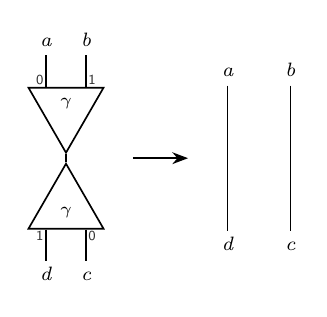
\begin{tikzpicture}[baseline=(current bounding box.center)]
  \cellD{t}{0,0.62}{$\gamma$}
  \cellU{b}{0,-0.62}{$\gamma$}
  \draw[wire] (t-p) -- (b-p);
  \draw[wire] (t-0) -- ++(0,0.4) node[port,above] {a};
  \draw[wire] (t-1) -- ++(0,0.4) node[port,above] {b};
  \draw[wire] (b-0) -- ++(0,-0.4) node[port,below] {c};
  \draw[wire] (b-1) -- ++(0,-0.4) node[port,below] {d};
  \draw[becomes] (0.85,0) -- (1.55,0);
  \node[port] (a) at (2.05,1.1) {a}; \node[port] (b) at (2.85,1.1) {b};
  \node[port] (d) at (2.05,-1.1) {d}; \node[port] (c) at (2.85,-1.1) {c};
  \draw[wire] (a) -- (d); \draw[wire] (b) -- (c);
\end{tikzpicture}
&
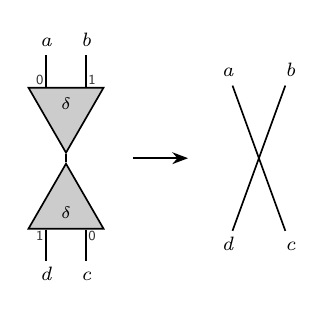
\begin{tikzpicture}[baseline=(current bounding box.center)]
  \cellD[isdup]{t}{0,0.62}{$\delta$}
  \cellU[isdup]{b}{0,-0.62}{$\delta$}
  \draw[wire] (t-p) -- (b-p);
  \draw[wire] (t-0) -- ++(0,0.4) node[port,above] {a};
  \draw[wire] (t-1) -- ++(0,0.4) node[port,above] {b};
  \draw[wire] (b-0) -- ++(0,-0.4) node[port,below] {c};
  \draw[wire] (b-1) -- ++(0,-0.4) node[port,below] {d};
  \draw[becomes] (0.85,0) -- (1.55,0);
  \node[port] (a) at (2.05,1.1) {a}; \node[port] (b) at (2.85,1.1) {b};
  \node[port] (d) at (2.05,-1.1) {d}; \node[port] (c) at (2.85,-1.1) {c};
  \draw[wire] (a) -- (c); \draw[wire] (b) -- (d);
\end{tikzpicture}
&
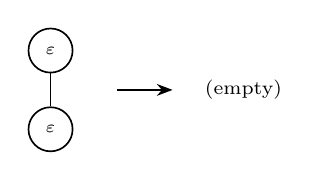
\begin{tikzpicture}[baseline=(current bounding box.center)]
  \node[eracell] (e) at (0,0.5) {$\varepsilon$};
  \node[eracell] (f) at (0,-0.5) {$\varepsilon$};
  \draw[wire] (e) -- (f);
  \draw[becomes] (0.85,0) -- (1.55,0);
  \node[font=\scriptsize] at (2.45,0) {(empty)};
\end{tikzpicture}
\\[0.6em]
\small $\gamma\gamma$: \cod{ruleConCon} & \small $\delta\delta$: \cod{ruleDupDup} &
\small $\varepsilon\varepsilon$: \cod{ruleEraEra}
\\[1.2em]
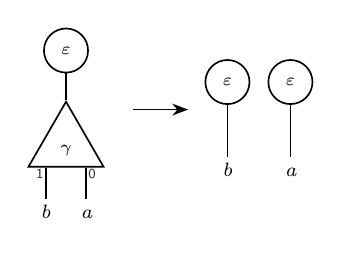
\begin{tikzpicture}[baseline=(current bounding box.center)]
  \node[eracell] (e) at (0,0.75) {$\varepsilon$};
  \cellU{b}{0,-0.45}{$\gamma$}
  \draw[wire] (e) -- (b-p);
  \draw[wire] (b-0) -- ++(0,-0.4) node[port,below] {a};
  \draw[wire] (b-1) -- ++(0,-0.4) node[port,below] {b};
  \draw[becomes] (0.85,0) -- (1.55,0);
  \node[eracell] (e1) at (2.05,0.35) {$\varepsilon$};
  \node[eracell] (e0) at (2.85,0.35) {$\varepsilon$};
  \draw[wire] (e1) -- ++(0,-0.95) node[port,below] {b};
  \draw[wire] (e0) -- ++(0,-0.95) node[port,below] {a};
\end{tikzpicture}
&
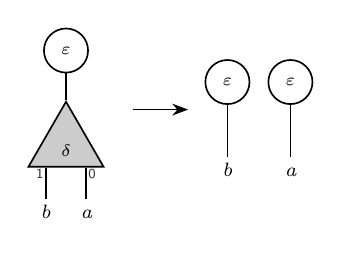
\begin{tikzpicture}[baseline=(current bounding box.center)]
  \node[eracell] (e) at (0,0.75) {$\varepsilon$};
  \cellU[isdup]{b}{0,-0.45}{$\delta$}
  \draw[wire] (e) -- (b-p);
  \draw[wire] (b-0) -- ++(0,-0.4) node[port,below] {a};
  \draw[wire] (b-1) -- ++(0,-0.4) node[port,below] {b};
  \draw[becomes] (0.85,0) -- (1.55,0);
  \node[eracell] (e1) at (2.05,0.35) {$\varepsilon$};
  \node[eracell] (e0) at (2.85,0.35) {$\varepsilon$};
  \draw[wire] (e1) -- ++(0,-0.95) node[port,below] {b};
  \draw[wire] (e0) -- ++(0,-0.95) node[port,below] {a};
\end{tikzpicture}
&
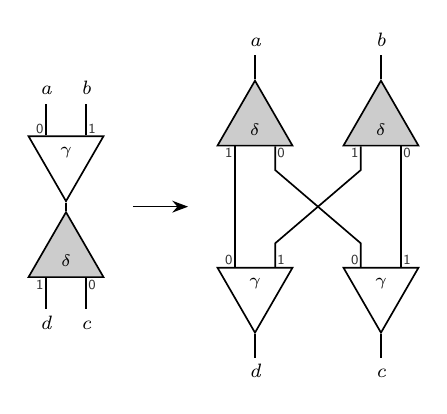
\begin{tikzpicture}[baseline=(current bounding box.center)]
  \cellD{t}{0,0.62}{$\gamma$}
  \cellU[isdup]{b}{0,-0.62}{$\delta$}
  \draw[wire] (t-p) -- (b-p);
  \draw[wire] (t-0) -- ++(0,0.4) node[port,above] {a};
  \draw[wire] (t-1) -- ++(0,0.4) node[port,above] {b};
  \draw[wire] (b-0) -- ++(0,-0.4) node[port,below] {c};
  \draw[wire] (b-1) -- ++(0,-0.4) node[port,below] {d};
  \draw[becomes] (0.85,0) -- (1.55,0);
  % a = dup(w0, w1), b = dup(w2, w3), c = con(w0, w2), d = con(w1, w3)
  \cellU[isdup]{da}{2.4,1.05}{$\delta$}
  \cellU[isdup]{db}{4.0,1.05}{$\delta$}
  \cellD{cd}{2.4,-1.05}{$\gamma$}
  \cellD{cc}{4.0,-1.05}{$\gamma$}
  \draw[wire] (da-p) -- ++(0,0.3) node[port,above] {a};
  \draw[wire] (db-p) -- ++(0,0.3) node[port,above] {b};
  \draw[wire] (cd-p) -- ++(0,-0.3) node[port,below] {d};
  \draw[wire] (cc-p) -- ++(0,-0.3) node[port,below] {c};
  \draw[wire] (da-0) -- ++(0,-0.3) -- ($(cc-0)+(0,0.3)$) -- (cc-0);
  \draw[wire] (da-1) -- (cd-0);
  \draw[wire] (db-0) -- (cc-1);
  \draw[wire] (db-1) -- ++(0,-0.3) -- ($(cd-1)+(0,0.3)$) -- (cd-1);
\end{tikzpicture}
\\[0.6em]
\small $\varepsilon\gamma$: \cod{ruleEraBin} & \small $\varepsilon\delta$: \cod{ruleEraBin} &
\small $\gamma\delta$: \cod{ruleConDup}
\end{tabular}

\caption{The six rules of the interaction combinators, drawn by hand from the Lean definitions
named under each rule ($\delta$ cells in grey). The small numbers are the indices of the
auxiliary ports in the code. The rules $\varepsilon\gamma$ and $\varepsilon\delta$ are one
definition. Compare \pp{Fig.~2, p.~81}.}
\label{fig:rules}
\end{figure}

\paragraph{The combinators.}
The symbols are $\gamma$ and $\delta$ of arity~2 and $\varepsilon$ of arity~0. There is one
rule for each of the six unordered pairs (Fig.~\ref{fig:rules}): three \emph{annihilations}
($\gamma\gamma$, $\delta\delta$, $\varepsilon\varepsilon$) and three \emph{commutations}
($\gamma\delta$, $\varepsilon\gamma$, $\varepsilon\delta$). The two annihilations of binary
cells differ: ``it is $\gamma\gamma$, not $\delta\delta$, which exchanges the ports''
\pp{p.~82}. In the code, $\gamma\gamma$ joins port $0$ of one cell to port $1$ of the other,
and $\delta\delta$ joins ports of the same index. With the clockwise convention, $\gamma\gamma$
is therefore drawn with straight wires and $\delta\delta$ with crossed wires. This asymmetry is used by the proof of universality (the transpositors of
Section~\ref{sec:components}), and the system in which both annihilations are alike is, in Lafont's
words, ``not universal in the technical sense of Theorem~1'' although it has the same
expressive power \pp{p.~97}.

%=================================================================================================
\section{Nets as text}
\label{sec:text}

Lafont remarks that a net can be described by sets of cells, wires and ports, and adds: ``In
this paper, we shall avoid such cumbersome descriptions, but the reader may check that our
arguments can always be formalized in this way'' \pp{p.~72}. We chose a description in which a
net is a piece of text, in the style of the interaction calculus of Fern\'andez and
Mackie~\cite{fernandezmackie1999}. The correspondence with graphs is proved in
Section~\ref{sec:graphs}.

\subsection{Trees, nets and equality}

Trees and nets are defined over a signature (an alphabet with its arities) and a type $\nu$ of
names.

\lean{term}
\lean{net}

A tree is a name or a cell together with a tree for each auxiliary port. The root of
\cod{app α ts} is the principal port of the cell (Fig.~\ref{fig:wire}a). A net is a multiset of
unordered pairs of trees (\cod{Sym2} is Mathlib's type of unordered pairs, and \cod{Fin n} the
type of the numbers below $n$). An equation $t = u$, written \cod{s(t, u)}, is a wire between
the root of $t$ and the root of $u$. A name is a wire as well: a name that occurs twice joins its
two occurrences, and a name that occurs once is a free port. A net is \emph{linear} when no
name occurs more than twice (\cod{N.vars} is the multiset of the occurrences of names in $N$).
Only linear texts are nets, and every theorem assumes linearity. A cyclic wire is the equation
$x = x$.

\begin{figure}[H]
\centering
% A cell, and two texts of the same graph that differ by one wire substitution.
\begin{tabular}{@{}c@{\hspace{1.4cm}}c@{\hspace{1.4cm}}c@{}}
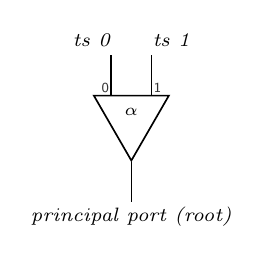
\begin{tikzpicture}[baseline=(current bounding box.center)]
  \cellD{c}{0,0}{$\alpha$}
  \draw[wire] (c-p) -- ++(0,-0.5) node[port,below] {principal port (root)};
  \draw[wire] (c-0) -- ++(0,0.5) node[port,above,xshift=-2.5mm] {ts 0};
  \draw[wire] (c-1) -- ++(0,0.5) node[port,above,xshift=2.5mm] {ts 1};
\end{tikzpicture}
&
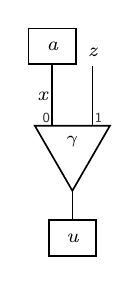
\begin{tikzpicture}[baseline=(current bounding box.center)]
  \cellD{c}{0,0}{$\gamma$}
  \node[boxtree] (u) at (0,-1.15) {u};
  \node[boxtree] (a) at ($(c-0)+(0,1.0)$) {a};
  \draw[wire] (c-p) -- (u.north);
  \draw[wire] (c-0) -- node[port,left] {x} (a.south);
  \draw[wire] (c-1) -- ++(0,0.75) node[port,above] {z};
\end{tikzpicture}
&
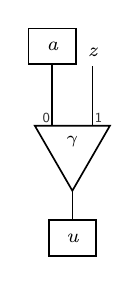
\begin{tikzpicture}[baseline=(current bounding box.center)]
  \cellD{c}{0,0}{$\gamma$}
  \node[boxtree] (u) at (0,-1.15) {u};
  \node[boxtree] (a) at ($(c-0)+(0,1.0)$) {a};
  \draw[wire] (c-p) -- (u.north);
  \draw[wire] (c-0) -- (a.south);
  \draw[wire] (c-1) -- ++(0,0.75) node[port,above] {z};
\end{tikzpicture}
\\[0.6em]
\small (a) \cod{app α ts}, arity 2 & \small (b) $u = \gamma(x, z),\ \ x = a$ &
\small (c) $u = \gamma(a, z)$
\end{tabular}

\caption{(a) A cell as the root of a tree. (b), (c) Two texts of the same graph: an equation is
a wire between two roots, and one step of \cod{Wire} takes (b) to (c).}
\label{fig:wire}
\end{figure}

The same graph has many texts: the equations $x = a$, $u = \gamma(x, z)$ and the single
equation $u = \gamma(a, z)$ describe the same net (Fig.~\ref{fig:wire}b, c). The relation
between them is one \emph{wire substitution}:

\lean{wire}

Here \cod{e ::ₘ Δ} is the multiset $\Delta$ with the equation $e$ added. The constructor says:
an equation $x = t$ is removed, and $t$ replaces the other occurrence of $x$, which lies in
another equation $a = b$. \Equiv{} is the equivalence relation generated by \cod{Wire}. It
plays the role of equality of nets, and it preserves linearity. It is kept apart from
reduction. A wire substitution performs no interaction: it preserves the multiset of cells and
the free ports. The statements of the paper count interactions (strong confluence closes a
diagram in one step on each side, a translation simulates $n$ steps in between $Ln$ and $Un$
steps), and those counts must not include bookkeeping. Results are therefore stated up to
\Equiv{}. A typical conclusion is ``reduces to a net that is \Equiv{} to this one''.

\subsection{Rules, reduction and interaction systems}

The right member of a rule between a cell with $a$ auxiliary ports and a cell with $b$ is a net
(\cod{Rule S a b}) whose names are the ports of the first cell, the ports of the second, and a
number of new wires: the name type is \cod{Fin a ⊕ Fin b ⊕ Fin internal}. Applying the rule
(\cod{r.inst as bs f}) plugs the trees \cod{as}, \cod{bs} into the port names and gives the
new wires the names \cod{f} in $\mathbb N$. A \cod{System S} gives, for each ordered pair of
symbols, at most one rule (\cod{I.rule α β} is \cod{some r} or \cod{none}). Since an equation
is unordered, a rule given for $\alpha$, $\beta$ also applies to $\beta$, $\alpha$.

\lean{step}

\cod{Step} is literal: the cut must be written as one equation between two cells, and
the new wires receive distinct names that do not occur in the net. It preserves linearity. \cod{StepE} first allows the
net to be rewritten into an equivalent text. It is needed because a cut of the graph
may be hidden behind a wire, as in $x = \alpha(\ldots)$, $x = \beta(\ldots)$. \cod{StepE} is
the reduction of graphs (Section~\ref{sec:graphs}, item~5), and Theorem~1 is stated with it.
\cod{Steps} and \cod{StepsE} are the reflexive-transitive closures.

\lean{symm}

\cod{WellFormed} collects Lafont's conditions on an interaction system. A right member is
linear (each port occurs once, each new wire twice) and reduced. \cod{Rule.Reduced} is a
syntactic form (every equation is $p = t$ with $p$ a port), related to the
semantic notion (no cut and no vicious circle in any equivalent text) by theorems in both
directions. A rule for $\alpha$, $\beta$ with $\alpha \neq \beta$ excludes one for $\beta$,
$\alpha$. A rule of a symbol with itself is symmetric: the paper asks that the right member
read from the other cell (\cod{r.swap}) be the same net, and the field \cod{symm} asks this up
to \Equiv{} and a permutation $\pi$ of the internal wires. The permutation is needed because
internal wires are named by \cod{Fin internal} and a wire substitution never renames a wire: a
right member such as $a = \beta(w_0, w_1)$, $b = \beta(w_1, w_0)$ is the same graph as its
swap, but the two texts are not \Equiv{}. (\cod{\_root\_.Equiv.Perm} is Mathlib's type of
permutations. The prefix is there because our \Equiv{} shadows Mathlib's.)

\subsection{Translations}

A principal net of arity $n$ (\cod{PNet}) is a tree in which each of $n$ ports occurs once and
each internal wire twice. This is the form that Proposition~2 of the paper gives to a principal
net. We take it as the definition, and do not prove that it agrees with the definition of
Section~\ref{sec:background}. A \cod{Translation S S'} gives a principal net over $S'$ of the
right arity for each symbol of $S$, and is \cod{Strict} when no such tree is a single name.
``$N'$ is a translation of $N$'' is a relation, \cod{Φ.NetTr N N'}, because each instance of a
principal net needs names for its internal wires. Every linear net has a translation, any two
are \Equiv{}, and equivalent nets have equivalent translations.

\lean{compatible}

\cod{Compatible} is the diagram of \pp{p.~81}. Here \cod{(Φ.net α).inst args f} is the
principal net of $\alpha$ with the trees \cod{args} on its ports and the names \cod{f} on its
internal wires. For every rule, and for all names \cod{xs}, \cod{ys} on the ports of the two
cells, the translations of the two cells plugged by their roots reduce to a net $M$ that is
\Equiv{} to a translation $N'$ of the right member, for some names $h$ of its new wires. The
definition quantifies over every naming for which the pair is a linear net, including namings
that join two ports of the same cell. It has no context: closure under context is part of the
proof of Proposition~4.

%=================================================================================================
\section{Text and graphs}
\label{sec:graphs}

This section states in what sense \Equiv{} and \cod{StepE} are equality and reduction of the
nets of the paper. The graph side follows Lafont's description \pp{p.~72}.

\lean{graph}

A graph has cells identified by natural numbers, wires that are unordered pairs of
\emph{ends}, and a number of cyclic wires. An end is a port of a cell (\cod{port c 0} is the
principal port, \cod{port c (i+1)} the $i$-th auxiliary port) or a name. A graph is well formed
when cells have distinct identities, every port of every cell ends exactly one wire, every end
that is a port belongs to a cell of the graph, and a name ends at most one wire (\cod{G.ends}
is the multiset of the ends of the wires of $G$). The names are then the free ports. Two graphs are isomorphic (\cod{Graph.Iso}) when they differ by the
identities of their cells.

The graph of a text is defined in two stages (Fig.~\ref{fig:graph}). The raw graph is read off
the text: one cell for each cell of the trees, one wire for each equation and one for each
auxiliary port. In it a name ends one wire per occurrence. Then every name that ends two wires
is erased, by joining the two wires or, for a wire from a name to itself, by turning it into a
cyclic wire. \cod{N.HasGraph G} says that $G$ is obtained from $N$ in this way.

\begin{figure}[H]
\centering
% The net con(x, y) = dup(x, y) of Checks/Core/GraphCheck.lean: raw graph and graph.
\begin{tabular}{@{}c@{\hspace{2.0cm}}c@{}}
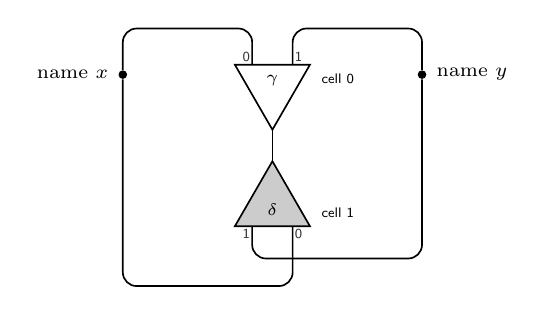
\begin{tikzpicture}[baseline=(current bounding box.center)]
  \cellD{c}{0,0.75}{$\gamma$}
  \cellU[isdup]{d}{0,-0.75}{$\delta$}
  \node[font=\tiny\sffamily,anchor=west] at ($(c.center)+(0.5,0.1)$) {cell 0};
  \node[font=\tiny\sffamily,anchor=west] at ($(d.center)+(0.5,-0.1)$) {cell 1};
  \draw[wire] (c-p) -- (d-p);
  \node[nm,label={[font=\scriptsize]left:name $x$}] (n0) at (-1.9,0.9) {};
  \node[nm,label={[font=\scriptsize]right:name $y$}] (n1) at (1.9,0.9) {};
  \draw[wire,rounded corners=5pt] (c-0) -- ++(0,0.45) -| (n0);
  \draw[wire,rounded corners=5pt] (c-1) -- ++(0,0.45) -| (n1);
  \draw[wire,rounded corners=5pt] (d-0) -- ++(0,-0.75) -| (n0);
  \draw[wire,rounded corners=5pt] (d-1) -- ++(0,-0.4) -| (n1);
\end{tikzpicture}
&
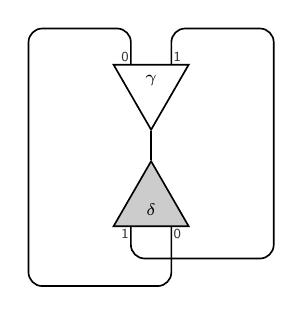
\begin{tikzpicture}[baseline=(current bounding box.center)]
  \cellD{c}{0,0.75}{$\gamma$}
  \cellU[isdup]{d}{0,-0.75}{$\delta$}
  \draw[wire] (c-p) -- (d-p);
  \draw[wire,rounded corners=5pt] (c-0) -- ++(0,0.45) -- ++(-1.3,0) |- ($(d-0)+(0,-0.75)$) -- (d-0);
  \draw[wire,rounded corners=5pt] (c-1) -- ++(0,0.45) -- ++(1.3,0) |- ($(d-1)+(0,-0.4)$) -- (d-1);
\end{tikzpicture}
\\[0.8em]
\small (a) the raw graph: 2 cells, 5 wires & \small (b) the graph: 2 cells, 3 wires
\end{tabular}

\caption{The net $\gamma(x, y) = \delta(x, y)$. (a) The raw graph read off the text: the wire
of the equation between the two principal ports, and a wire from each auxiliary port to its
name. Each name ends two wires. (b) After two contractions no name is left: the graph has two
cells, three wires and no free port.}
\label{fig:graph}
\end{figure}

Five statements are proved.

\begin{enumerate}
\item Every net has a graph, and that graph is well formed (\cod{graph\_exists}).
\item Two graphs of a linear net are isomorphic (\cod{graph\_unique}). They can differ by the
  identities of the cells and by the order of the contractions.
\item Two linear nets are \Equiv{} if and only if their graphs are isomorphic:
  \lean{graph_equiv}
\item Every well-formed graph is, up to isomorphism, the graph of a linear net with the same
  free ports (\cod{graph\_of\_net}, which gives a net for a graph).
\item \cod{StepE} is interaction of graphs, in both directions:
  \lean{graph_steps}
\end{enumerate}

In item~5, \cod{Graph.Interact} is defined on graphs: remove two cells joined by their
principal ports, add a copy of a graph of the right member with new cell identities, and
contract the names that now end two wires. \cod{LinearRules I} says that every right member is
linear. The direction from graphs to text in items~3 to~5 goes through a \emph{flat text} of a
graph: one equation for each cell, one equation between two names for each wire, and $x = x$
for each cyclic wire.

The results of the following sections are stated and proved on text. By the five statements
above they can be read as statements about graphs, but no corollary on graphs is derived in the
development, and item~5 is for single steps only. The statements are for our definition of a
graph, which was not compared with another formal definition of interaction nets, such as the
partial permutations of de Falco~\cite{defalco2010}.

%=================================================================================================
\section{Confluence, reduced nets and simulation}
\label{sec:theory}

The four propositions of~\cite[Section~1]{lafont1997} are in the development.

\paragraph{Proposition 1.}
If a net reduces in one step to $P$ and to $P'$ with $P \neq P'$, then $P$ and $P'$ reduce in
one step to a common $Q$ \pp{p.~73}.

\lean{prop1}

Lafont's hypothesis $P \neq P'$ becomes the alternative \cod{Equiv P P'}. For literal steps,
the case of two different cuts is the proof of the paper: they are two different equations and
the two rules apply independently. The case of the same cut of a symbol with itself, read from
either cell, is not in the paper's proof. It gives the same graph by the symmetry condition.
For \cod{StepE}, the two steps fire in two different texts $N_1$, $N_2$ of the same net, and a
cut of $N_2$ need not be an equation of $N_1$. Cells have no identity in a text. The proof
therefore describes a cut of a text as a chain of equations $\alpha(\vec a) = x_1$, $x_1 =
x_2$, $\ldots$, $x_k = \beta(\vec b)$, together with the net that firing it gives. Equivalent
texts have the same chains. Contracting the chain of the second cut in $N_1$ gives a text in
which both cuts are equations, and the literal theorem applies. It follows that a normal form is unique up to
\Equiv{} and that all reductions to it have the same number of steps
(\cod{normal\_form\_unique}).

\paragraph{Propositions 2 to 4.}
A net is \emph{reduced} if no equivalent text has an equation between two cells (a cut) or an
equation $x = t$ with $x$ a leaf of $t$ (a vicious circle). Proposition~2: a linear reduced net
is \Equiv{} to a net of trees hanging from its free ports, with their leaves joined by wires,
and two such nets that are \Equiv{} differ by an injective renaming that fixes the free ports
\pp{p.~79}. Proposition~3: a
translation of a reduced net is reduced, and conversely if the translation is strict
\pp{p.~80}. Proposition~4: if every rule is simulated in at least $L$ and at most $U$
interactions ($U$ is Lafont's $M$), then $n$ steps of the source are simulated in between $Ln$
and $Un$ interactions of the target \pp{p.~81}. Such bounds exist for a finite alphabet, and $L > 0$ for a strict
translation.

%=================================================================================================
\section{The universality proof}
\label{sec:universality}

This section follows~\cite[Section~2]{lafont1997}. Constructions are functions on trees:
\cod{mux ts} is the multiplexor $M_n$ with the trees \cod{ts} plugged into its $n$ auxiliary
ports. Their properties are stated in an arbitrary context $\Delta$. Those that erase or
duplicate also assume that the whole net is linear. In the statements, \cod{sig} and
\cod{system} are the signature and the system of the combinators, \cod{CNet} is the type of
nets over \cod{sig} with names in $\mathbb N$, and \cod{Red} is literal reduction
(\cod{Steps}) in \cod{system}.

\subsection{The components}
\label{sec:components}

The components of the paper are defined as in its figures, and each has the property the paper
states for it. We list them with the name of the theorem in \cod{Results.lean}.

\begin{itemize}
\item For $n \ge 1$ the multiplexor $M_n$ is a comb of $n - 1$ cells $\gamma$ ($M_0$ is an
  $\varepsilon$), and $M_n^*$ is its mirror image \pp{Fig.~4} (Fig.~\ref{fig:mux}). Plugged by
  their roots they reduce to $n$ wires in order, where \cod{Wires ts us} is the net of the
  equations $ts_i = us_i$:
  \lean{mux_prop}
\item The autodual multiplexor $T_n$ is the same comb built with $\delta$ \pp{Fig.~5}. The
  transpositor $T_{p,q}$ is $T_{p+q}$ with a $\gamma$ on each of its first $p$ ports (it has $2p + q$ ports), and
  every involution $\sigma$ has a transpositor $T_\sigma$: two copies plugged by their roots
  reduce to the wires $t_i = u_{\sigma(i)}$ \mbox{(\cod{transpositor\_property})}.
\item As text, a package is a tree in which every name occurs twice. An $\varepsilon$ erases a
  package (the corollary of Lemma~2 \pp{pp.~84--85}, \cod{lemma\_2\_erase\_package}). A menu is $M_n$ applied to $n$ packages,
  and the selector $S^i_n$ extracts the $i$-th and erases the others
  (\cod{menu\_selector\_property}).
\item A $\delta$ duplicates a package that contains no $\delta$ (the corollary of Lemma~3
  \pp{p.~87}, \cod{lemma\_3\_dup\_package}). The copier $C_n$ makes $n$ copies
  (\cod{copier\_property}). A copy is the package with its names renamed injectively. The
  restriction cannot be dropped: the package $\delta(x, x)$ plugged into a $\delta$ does not
  reduce to two copies of itself (\cod{dup\_package\_needs\_dupFree}, among the examples
  outside the library).
\item An arbitrary package $\pi$ has a code $!\pi$ that contains no $\delta$, and the decoder
  $D$ recovers $\pi$ from it \pp{Figs.~8 and~9} (\cod{decoder\_property}).
\end{itemize}

\begin{figure}[H]
\centering
% M_3, M_3^* and T_{1,1} as trees of cells, read off `mux`, `muxStar`, `transpositor 1`.
\begin{tabular}{@{}c@{\hspace{1.5cm}}c@{\hspace{1.5cm}}c@{}}
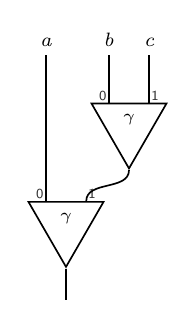
\begin{tikzpicture}[baseline=(current bounding box.center)]
  % mux [a, b, c] = con(a, con(b, c))
  \cellD{l}{0,0}{$\gamma$}
  \cellD{u}{0.8,1.25}{$\gamma$}
  \draw[wire] (l-p) -- ++(0,-0.4);
  \draw[wire] (l-1) to[out=90,in=-90] (u-p);
  \draw[wire] (l-0) -- ($(l-0)+(0,1.85)$) node[port,above] {a};
  \draw[wire] (u-0) -- ++(0,0.6) node[port,above] {b};
  \draw[wire] (u-1) -- ++(0,0.6) node[port,above] {c};
\end{tikzpicture}
&
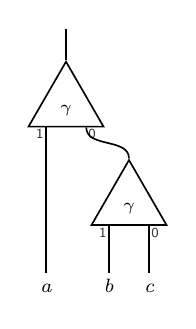
\begin{tikzpicture}[baseline=(current bounding box.center)]
  % muxStar [a, b, c] = con(con(c, b), a): cells pointing up, first port on the right
  \cellU{l}{0,0}{$\gamma$}
  \cellU{u}{0.8,-1.25}{$\gamma$}
  \draw[wire] (l-p) -- ++(0,0.4);
  % port 1 of the upper cell (drawn left) carries a; port 0 (drawn right) carries the lower cell
  \draw[wire] (l-1) -- ($(l-1)+(0,-1.85)$) node[port,below] {a};
  \draw[wire] (l-0) to[out=-90,in=90] (u-p);
  \draw[wire] (u-1) -- ++(0,-0.6) node[port,below] {b};
  \draw[wire] (u-0) -- ++(0,-0.6) node[port,below] {c};
\end{tikzpicture}
&
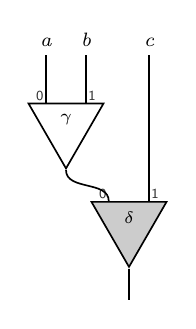
\begin{tikzpicture}[baseline=(current bounding box.center)]
  % transpositor 1 [a, b, c] = dup(con(a, b), c)
  \cellD[isdup]{l}{0,0}{$\delta$}
  \cellD{u}{-0.8,1.25}{$\gamma$}
  \draw[wire] (l-p) -- ++(0,-0.4);
  \draw[wire] (l-0) to[out=90,in=-90] (u-p);
  \draw[wire] (l-1) -- ($(l-1)+(0,1.85)$) node[port,above] {c};
  \draw[wire] (u-0) -- ++(0,0.6) node[port,above] {a};
  \draw[wire] (u-1) -- ++(0,0.6) node[port,above] {b};
\end{tikzpicture}
\\[0.6em]
\small $M_3$: \cod{mux [a, b, c]} & \small $M_3^*$: \cod{muxStar [a, b, c]} &
\small $T_{1,1}$: \cod{transpositor 1 [a, b, c]}
\end{tabular}

\caption{$M_3$, $M_3^*$ and the transpositor $T_{1,1}$ as trees of cells, read off the
definitions. Compare \pp{Fig.~4 and p.~83}.}
\label{fig:mux}
\end{figure}

\subsection{Decomposition of a rule}
\label{sec:decomp}

The right member of a rule for $\alpha_i$, $\alpha_j$ is cut into a net $\varphi_{i,j}$ on the
ports of $\alpha_i$, a net $\psi_{i,j}$ on the ports of $\alpha_j$, and a permutation
$\sigma_{i,j}$ of the $k$ wires in the middle \pp{p.~85}. In Lean a side is itself a rule,
whose second group of ports are the middle wires. \cod{plug} puts two sides back together,
joining the middle wire $l$ of $\varphi$ to the middle wire $\sigma(l)$ of $\psi$, and a
decomposition is correct for a rule when plugging gives the rule back up to \Equiv{} and an
injective renaming of its internal wires.

The translation needs a symmetric normal form: for the rule of a symbol with itself, $\varphi =
\psi$ and $\sigma$ is an involution, because the two cells of the cut are translated by
the same net and must each contribute the same half. In the paper, $\varphi_{j,i} =
\psi_{i,j}$ and $\sigma_{j,i} = \sigma_{i,j}^{-1}$ follow ``by the symmetry condition, and by
uniqueness of the canonical decomposition'' \pp{p.~85}. The paper does not define the
canonical decomposition. It states that one exists and shows it for one rule. The picture
suggests the decomposition of Proposition~2 (trees at the ports of each cell, the wiring as
$\sigma$), but the order of the middle wires, on which the uniqueness of $\sigma$ depends, is
not specified. Mazza's thesis~\cite{mazza2006} repeats the argument, referring to Lafont for the
canonical decomposition, and we know of no source that defines it.

The obvious decomposition of a text, \cod{Rule.decompose},
sends the equations rooted at a port of the first cell to $\varphi$ and the others to $\psi$,
and numbers the middle wires by their names in the text. It is correct for every linear rule.
But for the rule of a ternary symbol with itself
\begin{align*}
  a_0 &= \gamma(w_0, w_1), & a_1 &= \gamma(w_2, \varepsilon), & a_2 &= w_3,\\
  b_0 &= \gamma(w_2, w_1), & b_1 &= \gamma(w_0, \varepsilon), & b_2 &= w_3,
\end{align*}
which is linear, reduced and symmetric, it gives the permutation $\sigma = (2, 0, 1, 3)$ of the
four middle wires, which is not an involution, and $\varphi \neq \psi$. The decomposition
depends on the text of the rule and not only on its graph. We did not formalize a decomposition
defined on graphs.

The normal form is obtained differently. A net is in \emph{expanded form} when every equation
is $p = t$ with $p$ a port and every leaf of $t$ an internal wire. Every linear reduced rule
has an expanded form, and expanded nets are rigid: two linear expanded nets with the same
number of internal wires that are \Equiv{} differ by a permutation of those wires. For the rule
of a symbol with itself, the symmetry condition then becomes a permutation of the internal
wires of the expanded rule, from which a symmetric decomposition is read. For two different
symbols, the obvious decomposition is used and $\sigma$ is moved into $\varphi$, so that
$\sigma$ is the identity. The outcome is \cod{System.exists\_decData}: every well-formed
system has, for each rule, two linear reduced sides and an involution that plug back into the
rule, with $\varphi = \psi$ for a symbol with itself. The sides are then put in expanded form,
so that the tree of a side at each port can be read off, and they still plug back
(\cod{System.DecData.sidesPlug}). The rest of the proof uses only this property of a family
of sides, where \cod{side α β} is the side of $\alpha$ in its rule with $\beta$:

\lean{sidesplug}

\subsection{The translation}
\label{sec:general}

A system is recursion-free when the symbols can be ordered and the rules decomposed so that
$\varphi_{i,j}$ contains only symbols strictly smaller than $\alpha_j$, and $\psi_{i,j}$ only
symbols strictly smaller than $\alpha_i$ \pp{p.~86}. For such a system the cell $[\alpha_i]$
of \pp{Fig.~6} is a transpositor $T_{1,1}$ carrying a menu $\Gamma_i = \Gamma_{1,i} \,\&\,
\cdots \,\&\, \Gamma_{m,i}$ (the multiplexor $M_m$ applied to these packages), the selector
$S^i_m$, and a multiplexor $M_{n_i+1}$ on the ports of the cell. The package $\Gamma_{i,j}$,
which $\alpha_i$ selects from the menu of $\alpha_j$, contains the translation of
$\varphi_{i,j}$. This case is in the
development (\cod{recursion\_free\_compatible}), with its termination
(\cod{recursion\_free\_terminates}).

In general the packages of $[\alpha_i]$ cannot contain $[\alpha_k]$ for the symbols of its
right members, since the definition would be circular. Each
cell carries instead a code $!\Gamma$ of the menus of all symbols \pp{Fig.~10}, from
which the translation of any cell is rebuilt when a rule fires (Fig.~\ref{fig:cell}). The
packages $\Gamma_{i,j}$ contain, in place of a translated cell, a cell
$\langle\alpha_k\rangle$ with one extra port: on that port a copier $C_2$ receives a copy of
$!\Gamma$, sends one copy to a decoder followed by the selector $S^k_m$, which delivers
$\Gamma_k$, and keeps the other as the code of the rebuilt cell. The package $\Gamma_{i,j}$ is a multiplexor $M^*_{n_i+2}$ whose first leaf is a copier $C_p$,
which distributes $!\Gamma$ to the $p$ cells of $\langle\varphi_{i,j}\rangle$, followed by the
trees of $\langle\varphi_{i,j}\rangle$ at the ports of $\alpha_i$ and, as last leaf, by
$T_{\sigma_{i,j}}$ on its middle ports. In Lean
the translation is a function \cod{codeTranslationE e side} of a numbering \cod{e} of the
symbols and a family \cod{side} of sides. It is strict, since the root of $[\alpha]$ is a
$\delta$.

\begin{figure}[H]
\centering
% Schematic of the principal net [alpha] of the general translation (`codeTreeE`), as a tree of
% named components. Our own block diagram; it is not a reproduction of Lafont's Fig. 10.
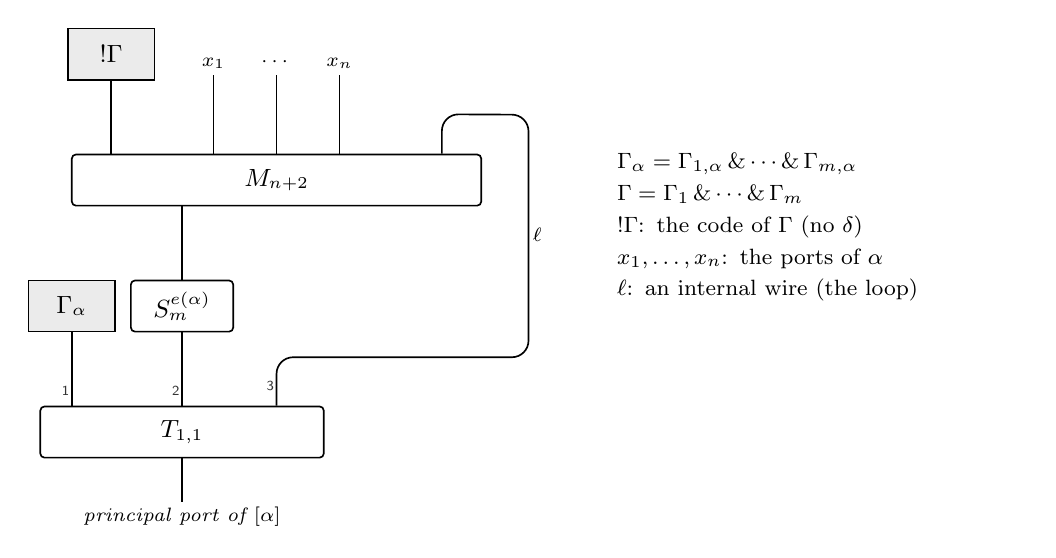
\begin{tikzpicture}[
    blk/.style={draw,line width=0.6pt,rounded corners=1.5pt,minimum height=6.5mm,
      minimum width=13mm,inner sep=2pt,font=\small},
    pk/.style={draw,line width=0.6pt,minimum height=6.5mm,minimum width=11mm,inner sep=2pt,
      font=\small,fill=black!8}]
  \node[blk,minimum width=36mm] (T) at (0,0) {$T_{1,1}$};
  \draw[wire] (T.south) -- ++(0,-0.55) node[port,below] {principal port of $[\alpha]$};
  \node[pk] (G) at (-1.4,1.6) {$\Gamma_\alpha$};
  \node[blk] (S) at (0,1.6) {$S^{e(\alpha)}_m$};
  \node[blk,minimum width=52mm] (M) at (1.2,3.2) {$M_{n+2}$};
  \node[pk] (C) at (-0.9,4.8) {$!\Gamma$};
  \draw[wire] (G.south) -- node[idx,left,pos=0.8] {1} (G.south |- T.north);
  \draw[wire] (S.south) -- node[idx,left,pos=0.8] {2} (T.north);
  \draw[wire] (S.north) -- (S.north |- M.south);
  \draw[wire] (C.south) -- (C.south |- M.north);
  \foreach \x/\l in {0.4/{x_1},1.2/{\cdots},2.0/{x_n}} {
    \draw[wire] (\x,0 |- M.north) -- ++(0,1.0) node[port,above] {$\l$};}
  \draw[wire,rounded corners=6pt] (3.3,0 |- M.north) -- ++(0,0.5) -- (4.4,4.03) -- (4.4,0.95)
    node[port,right,pos=0.5] {$\ell$} -- (1.2,0.95) -- node[idx,left,pos=0.6] {3} (1.2,0 |- T.north);
  \node[font=\footnotesize,anchor=west,text width=5.1cm] at (5.4,2.6)
    {$\Gamma_\alpha=\Gamma_{1,\alpha}\,\&\cdots\&\,\Gamma_{m,\alpha}$\\[2pt]
     $\Gamma=\Gamma_1\,\&\cdots\&\,\Gamma_m$\\[2pt]
     $!\Gamma$: the code of $\Gamma$ (no $\delta$)\\[2pt]
     $x_1,\dots,x_n$: the ports of $\alpha$\\[2pt]
     $\ell$: an internal wire (the loop)};
\end{tikzpicture}

\caption{The principal net $[\alpha]$ of the general translation as a tree of components, for
a symbol $\alpha$ of arity $n$ in an alphabet of $m$ symbols numbered by $e$. The numbers 1 to
3 are the ports of $T_{1,1}$ in the order of the figure of the paper. Shaded boxes are
packages. Compare \pp{Fig.~10, top left}.}
\label{fig:cell}
\end{figure}

\subsection{The analogue of Fig.~7}
\label{sec:reader}

Fix a rule for $\alpha$, $\beta$ with sides $\varphi$ and $\psi$ sharing $k$ middle wires and
the involution $\sigma$ (the identity when $\alpha \neq \beta$, in which case $T_\sigma$ is an
autodual multiplexor), names $\vec x$, $\vec y$ on the ports of the two cells, and a context
$\Delta$ such that the whole net is linear. The starting net is $[\alpha](\vec x) =
[\beta](\vec y)$ beside $\Delta$. The lemmas carry the context $\Delta$, and the final
statement takes it empty. The proof has four reductions, their composition, and a conclusion
(Fig.~\ref{fig:reader} and Table~\ref{tab:reader}).

\begin{figure}[H]
\centering
% The reduction of two translated cells [alpha] = [beta] of the general translation, in five
% nets: the analogue of Lafont's Fig. 7. Our own block diagram, drawn from the six steps of
% Section 6.4. A wire with a stroke across it is a bundle of wires.
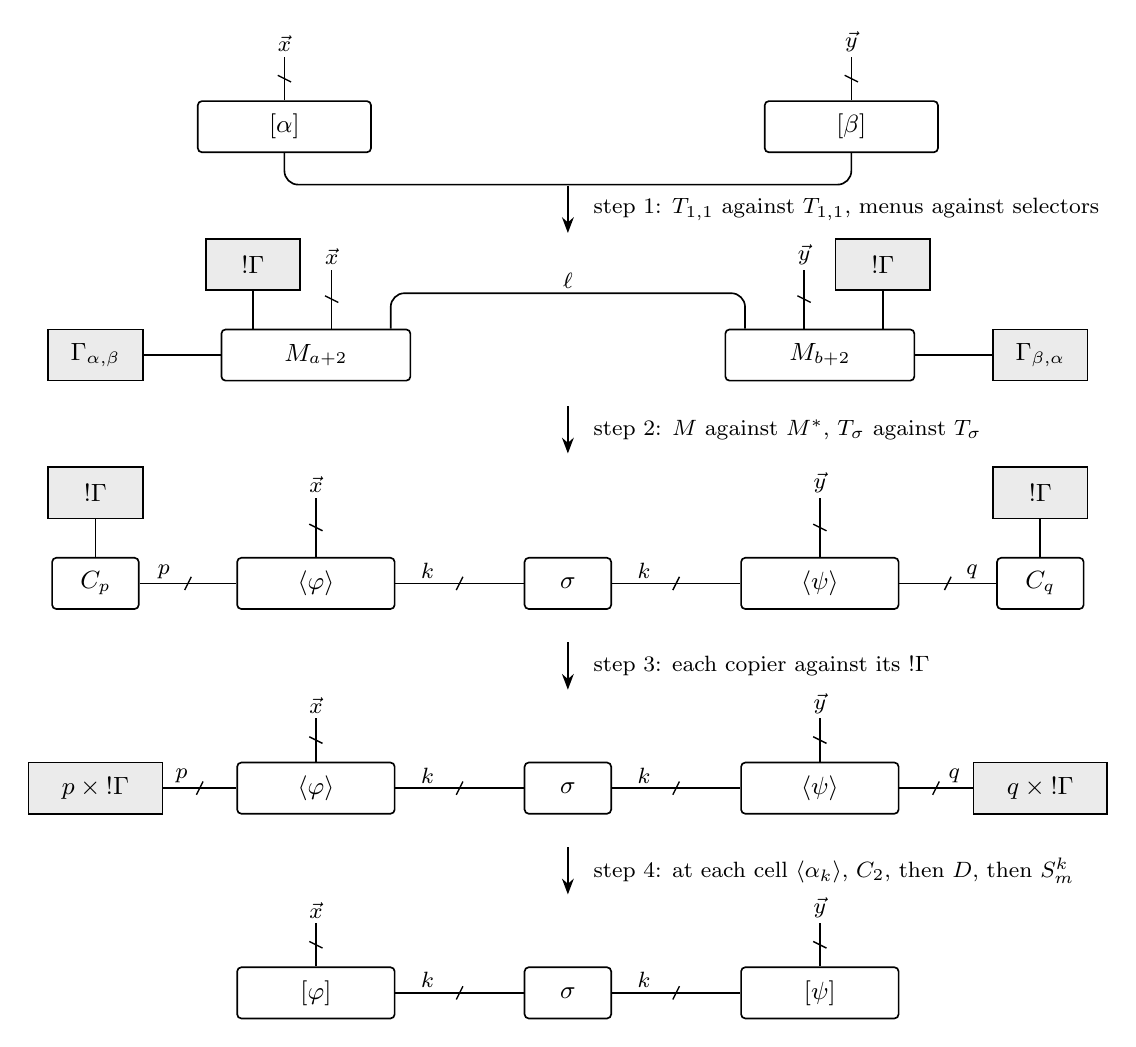
\begin{tikzpicture}[
    blk/.style={draw,line width=0.6pt,rounded corners=1.5pt,minimum height=6.5mm,
      minimum width=14mm,inner sep=2pt,font=\small},
    pk/.style={draw,line width=0.6pt,minimum height=6.5mm,minimum width=12mm,inner sep=2pt,
      font=\small,fill=black!8},
    lab/.style={font=\footnotesize,inner sep=1.5pt},
    stp/.style={font=\footnotesize,anchor=west,inner sep=2pt},
    bundle/.style={postaction={decorate,decoration={markings,
      mark=at position 0.5 with {\draw[line width=0.5pt] (-1.2pt,-2.4pt) -- (1.2pt,2.4pt);}}}}]
  % ---------------------------------------------------------------- net 1: the two cells
  \node[blk,minimum width=22mm] (A1) at (3.4,0) {$[\alpha]$};
  \node[blk,minimum width=22mm] (B1) at (10.6,0) {$[\beta]$};
  \draw[wire,bundle] (A1.north) -- ++(0,0.55) node[lab,above] {$\vec x$};
  \draw[wire,bundle] (B1.north) -- ++(0,0.55) node[lab,above] {$\vec y$};
  \draw[wire,rounded corners=5pt] (A1.south) -- ++(0,-0.4) -| (B1.south);
  % ---------------------------------------------------------------- net 2: after step 1
  \begin{scope}[yshift=-2.9cm]
    \node[pk] (G2) at (1.0,0) {$\Gamma_{\alpha,\beta}$};
    \node[blk,minimum width=24mm] (M2) at (3.8,0) {$M_{a+2}$};
    \node[blk,minimum width=24mm] (N2) at (10.2,0) {$M_{b+2}$};
    \node[pk] (H2) at (13.0,0) {$\Gamma_{\beta,\alpha}$};
    \node[pk] (C2) at (3.0,1.15) {$!\Gamma$};
    \node[pk] (D2) at (11.0,1.15) {$!\Gamma$};
    \draw[wire] (G2.east) -- (M2.west);
    \draw[wire] (H2.west) -- (N2.east);
    \draw[wire] (C2.south) -- (C2.south |- M2.north);
    \draw[wire] (D2.south) -- (D2.south |- N2.north);
    \draw[wire,bundle] (4.0,0 |- M2.north) -- ++(0,0.75) node[lab,above] {$\vec x$};
    \draw[wire,bundle] (10.0,0 |- N2.north) -- ++(0,0.75) node[lab,above] {$\vec y$};
    \draw[wire,rounded corners=5pt] (4.75,0 |- M2.north) -- ++(0,0.45) -|
      node[lab,above,pos=0.25] {$\ell$} (9.25,0 |- N2.north);
  \end{scope}
  % ---------------------------------------------------------------- net 3: after step 2
  \begin{scope}[yshift=-5.8cm]
    \node[blk,minimum width=11mm] (P3) at (1.0,0) {$C_p$};
    \node[pk] (C3) at (1.0,1.15) {$!\Gamma$};
    \node[blk,minimum width=20mm] (F3) at (3.8,0) {$\langle\varphi\rangle$};
    \node[blk,minimum width=11mm] (S3) at (7.0,0) {$\sigma$};
    \node[blk,minimum width=20mm] (Y3) at (10.2,0) {$\langle\psi\rangle$};
    \node[blk,minimum width=11mm] (Q3) at (13.0,0) {$C_q$};
    \node[pk] (D3) at (13.0,1.15) {$!\Gamma$};
    \draw[wire] (C3.south) -- (P3.north);
    \draw[wire] (D3.south) -- (Q3.north);
    \draw[wire,bundle] (P3.east) -- node[lab,above,pos=0.25] {$p$} (F3.west);
    \draw[wire,bundle] (Q3.west) -- node[lab,above,pos=0.25] {$q$} (Y3.east);
    \draw[wire,bundle] (F3.east) -- node[lab,above,pos=0.25] {$k$} (S3.west);
    \draw[wire,bundle] (S3.east) -- node[lab,above,pos=0.25] {$k$} (Y3.west);
    \draw[wire,bundle] (F3.north) -- ++(0,0.75) node[lab,above] {$\vec x$};
    \draw[wire,bundle] (Y3.north) -- ++(0,0.75) node[lab,above] {$\vec y$};
  \end{scope}
  % ---------------------------------------------------------------- net 4: after step 3
  \begin{scope}[yshift=-8.4cm]
    \node[pk,minimum width=17mm] (C4) at (1.0,0) {$p\times{!\Gamma}$};
    \node[blk,minimum width=20mm] (F4) at (3.8,0) {$\langle\varphi\rangle$};
    \node[blk,minimum width=11mm] (S4) at (7.0,0) {$\sigma$};
    \node[blk,minimum width=20mm] (Y4) at (10.2,0) {$\langle\psi\rangle$};
    \node[pk,minimum width=17mm] (D4) at (13.0,0) {$q\times{!\Gamma}$};
    \draw[wire,bundle] (C4.east) -- node[lab,above,pos=0.25] {$p$} (F4.west);
    \draw[wire,bundle] (D4.west) -- node[lab,above,pos=0.25] {$q$} (Y4.east);
    \draw[wire,bundle] (F4.east) -- node[lab,above,pos=0.25] {$k$} (S4.west);
    \draw[wire,bundle] (S4.east) -- node[lab,above,pos=0.25] {$k$} (Y4.west);
    \draw[wire,bundle] (F4.north) -- ++(0,0.55) node[lab,above] {$\vec x$};
    \draw[wire,bundle] (Y4.north) -- ++(0,0.55) node[lab,above] {$\vec y$};
  \end{scope}
  % ---------------------------------------------------------------- net 5: after step 4
  \begin{scope}[yshift=-11.0cm]
    \node[blk,minimum width=20mm] (F5) at (3.8,0) {$[\varphi]$};
    \node[blk,minimum width=11mm] (S5) at (7.0,0) {$\sigma$};
    \node[blk,minimum width=20mm] (Y5) at (10.2,0) {$[\psi]$};
    \draw[wire,bundle] (F5.east) -- node[lab,above,pos=0.25] {$k$} (S5.west);
    \draw[wire,bundle] (S5.east) -- node[lab,above,pos=0.25] {$k$} (Y5.west);
    \draw[wire,bundle] (F5.north) -- ++(0,0.55) node[lab,above] {$\vec x$};
    \draw[wire,bundle] (Y5.north) -- ++(0,0.55) node[lab,above] {$\vec y$};
  \end{scope}
  % ---------------------------------------------------------------- the steps
  \draw[becomes] (7.0,-0.75) -- (7.0,-1.35);
  \node[stp] at (7.25,-1.05) {step 1: $T_{1,1}$ against $T_{1,1}$, menus against selectors};
  \draw[becomes] (7.0,-3.55) -- (7.0,-4.15);
  \node[stp] at (7.25,-3.85) {step 2: $M$ against $M^*$, $T_\sigma$ against $T_\sigma$};
  \draw[becomes] (7.0,-6.55) -- (7.0,-7.15);
  \node[stp] at (7.25,-6.85) {step 3: each copier against its $!\Gamma$};
  \draw[becomes] (7.0,-9.15) -- (7.0,-9.75);
  \node[stp] at (7.25,-9.45) {step 4: at each cell $\langle\alpha_k\rangle$, $C_2$, then $D$,
    then $S^k_m$};
\end{tikzpicture}

\caption{The analogue of \pp{Fig.~7} for the general translation, as a block diagram. A wire
with a stroke is a bundle of wires. $\langle\varphi\rangle$ stands for the trees of the side
$\varphi$ with a cell $\langle\alpha_k\rangle$ in place of each cell, $[\varphi]$ for their
translations, and $\sigma$ for the wiring that joins the middle port $l$ of $\varphi$ to the
middle port $\sigma(l)$ of $\psi$. The last net is the translation of the right member
(steps 5 and 6).}
\label{fig:reader}
\end{figure}

\begin{enumerate}
\item \emph{The two cells meet.} The two $T_{1,1}$ annihilate. The $\gamma\gamma$ step
  exchanges ports, so the menu of each cell faces the selector of the other, and the two loops
  become one wire $\ell$. Each selector extracts one package and erases the others. Two
  equations remain: the multiplexor of $[\alpha]$, with leaves $!\Gamma$, $\vec x$, $\ell$,
  against $\Gamma_{\alpha,\beta}$, and the multiplexor of $[\beta]$, with leaves $!\Gamma$,
  $\vec y$ and the same $\ell$, against $\Gamma_{\beta,\alpha}$.
\item \emph{The multiplexors annihilate} with the dual multiplexors at the roots of the
  packages. Leaf by leaf: $!\Gamma$ faces the copier $C_p$, each port $x_i$ faces the tree of
  $\langle\varphi\rangle$ at port $i$, and $\ell$ faces $T_\sigma$. The two transpositors
  $T_\sigma$, joined by $\ell$, annihilate: the tree of $\langle\varphi\rangle$ at the middle
  port $l$ faces the tree of $\langle\psi\rangle$ at $\sigma(l)$.
\item \emph{The copier duplicates the code.} $!\Gamma$ is a package without $\delta$, so $C_p$
  makes $p$ renamed copies of it, one on the extra port of each cell of
  $\langle\varphi\rangle$.
\item \emph{Each cell is rebuilt from its copy of the code}, by induction on the tree. At a
  cell $\langle\alpha_k\rangle$ the copier $C_2$ duplicates the copy of $!\Gamma$, the decoder
  turns one copy back into $\Gamma$, and the selector extracts $\Gamma_k$. The result is a
  renamed copy of the tree of $[\alpha_k]$, and a separate lemma shows that it is an instance
  of the principal net $[\alpha_k]$.
\item \emph{The result is the end of Lafont's Fig.~7}: the net of the equations $x_p =
  t_\varphi(p)$, $y_q = t_\psi(q)$ and $t_\varphi(l) = t_\psi(\sigma(l))$, where $t_\varphi$,
  $t_\psi$ are translations of the trees of the two sides. In Lean, with \cod{codeNetE e side α}
  for $[\alpha]$, \cod{plugTermTarget} for that net and \cod{gammaTree φ k₀ p} for the tree of
  $\varphi$ at $p$:
  \lean{cells_plug}
\item \emph{It is a translation of the right member.} The net of step~5 is a translation of
  $\varphi$ plugged into $\psi$ through $\sigma$. Since the sides plug back into the rule and
  translations respect \Equiv{}, it is \Equiv{} to a translation of an instance of the rule.
\end{enumerate}

\begin{table}[H]
\centering\small
\begin{tabular}{@{}llp{8.0cm}@{}}
\toprule
Step & Lemma & Interactions performed \\
\midrule
1 & \cod{codeCells\_meetE} & $T_{1,1}$ against $T_{1,1}$, two menus against two selectors \\
2 & \cod{codeCells\_meet\_endE} & $M_{a+2}$, $M_{b+2}$ against their duals, $T_\sigma$ against
  $T_\sigma$ \\
3 & \cod{codeGamma\_extractE} & $C_p$ against $!\Gamma$, on each side \\
4 & \cod{codeTerm\_extractE} & at each cell: $C_2$ against a copy of $!\Gamma$, the code
  against $D$, a menu against $S^k_m$ \\
5 & \cod{codeCells\_plugE} & (composition of steps 1 to 4) \\
6 & \cod{codeTranslationE\_compatible\_of\_sides} & none \\
\bottomrule
\end{tabular}
\caption{The analogue of \pp{Fig.~7} for the translation of \pp{Fig.~10}: the steps of the
proof, the Lean lemma for each, and the interactions it performs. The suffix \texttt{E} marks
statements for the translation given by data (Section~\ref{sec:thm}).}
\label{tab:reader}
\end{table}

The pictures do not show names. Every copy made by a copier is a renamed copy, so step~4 has to
show that a tree assembled from two differently renamed copies and a block of fresh names is an
instance of one fixed principal net. The pictures also do not show the order of reduction. The
cells of $\langle\varphi\rangle$ are rebuilt one at a time, each beside all the others and
beside the copies not yet consumed, so every lemma carries a context.

\subsection{The theorem}
\label{sec:thm}

The statement, as it stands in \cod{Results.lean}:

\lean{thm1}

The hypothesis \cod{[Finite S.Sym]} is the paper's: an alphabet is finite. The proof takes
sides from \cod{System.exists\_decData} and applies step~6. Strictness is not in the statement
of Theorem~1 in the paper, but Lafont's translation is strict. \cod{Compatible} allows a rule
to be simulated in zero steps. The bounded form is \cod{theorem\_1\_bounds}: there are $L > 0$
and $U$ such that every rule is simulated in at least $L$ and at most $U$ interactions. The
bounds are shown to exist and are not computed.

The statement depends on the definitions of trees, nets, linearity, \cod{Wire} and \Equiv{},
rules and their instances, systems and \cod{WellFormed}, \cod{Step} and \cod{StepsE}, principal
nets, translations, \cod{NetTr} and \cod{Compatible}, and on the six rules of the combinators.
These are what a reader has to check in order to trust it. The development uses Lean
\cod{v4.36.0} and Mathlib \cod{v4.36.0}, no axiom beyond the three standard ones of Lean
(\cod{propext}, \cod{Classical.choice}, \cod{Quot.sound}), and no \cod{native\_decide}.

The theorem can also be stated with the decomposition given as data. Given a numbering of the
symbols and a family of sides that plug back into the rules (\cod{SidesPlug},
Section~\ref{sec:decomp}), the translation is strict and compatible. The conditions on the
system serve to produce such sides:

\lean{thm1_explicit}

In this form nothing is chosen by the axiom of choice, and the translation is a Lean function
that can be evaluated. For unary addition (symbols $0$, $S$ and \cod{add}, two rules, one of
them recursive), with sides written by hand, evaluating the principal nets $[0]$, $[S]$ and
$[\mathtt{add}]$ gives 93, 128 and 95 cells. Each carries the code of the menus of all three
symbols. The development also proves, for unary addition and for the multiplication of
\pp{Section~1.5}, that the translations of the nets of $2 + 2$ and $2 \times 2$ reduce in the
combinators to translations of the net of $4$. This follows from the theorem and
Proposition~4. No reduction of a translated net was run.

%=================================================================================================
\section{The formalization process}
\label{sec:method}

The definitions of Section~\ref{sec:text} and the statement of Theorem~1 were written by the
author, with an AI assistant, before any proof existed, and were then fixed: no agent could
change them. The graph definitions of Section~\ref{sec:graphs} were written by the author in the
same way, after Theorem~1 had been proved, except the definition of interaction on graphs, which
was written by an agent. The file \cod{Results.lean}, from which the boxed statements of this
paper are quoted, was written by the author and restates theorems of the library that were
stated and proved by agents. After Theorem~1 had been proved, every definition taken from a
figure of \pp{Sections~2.1 to~2.7} was compared with its figure, wire by wire, under the port
convention of Section~\ref{sec:background}. Finally the author reviewed again the statements of
the main results, and the definitions they depend on, against the paper.

The proofs were written by a swarm of autonomous language-model agents, at most two running at
a time, with no human answering their questions. A planning agent turned a roadmap into tasks,
each asking for one lemma or for the review of one definition. A working agent took a task,
wrote Lean on its own branch, and submitted it. A reviewing agent, given a definition written
by another, compared it with the page of the paper and tried to refute the statements about
it, leaving its examples and counterexamples as Lean files outside the library. A submission
was merged automatically when it passed one script: no change to a fixed file, no \cod{sorry}
or added axiom, a full build, and an audit that every theorem depends only on the three
standard axioms of Lean. Table~\ref{tab:numbers} gives the size of the run. Of the 529
sessions, 229 belong to a last phase that only changed the layout of the source files.

\begin{table}[ht]
\centering\small
\begin{tabular}{@{}lr@{}}
\toprule
Agent sessions & 529 \\
Total session time & 51.9\,h \\
Wall-clock time of the three runs of the swarm & 29.8\,h \\
From the first agent to the proof of Theorem~1 & 8\,h 57\,min \\
Contributions merged & 301 \\
Lean, library & $44\,835$ lines \\
Lean, examples and counterexamples & $22\,434$ lines \\
Lean, worked examples (addition, multiplication) & $2\,202$ lines \\
\bottomrule
\end{tabular}
\caption{The size of the run and of the development.}
\label{tab:numbers}
\end{table}

Two definitions were corrected after Theorem~1 had been proved. The symmetry condition on the
rule of a symbol with itself was at first stated as \Equiv{} between the right member and its
swap. A reviewing agent exhibited an interaction system that this excludes (the rule shown in
Section~\ref{sec:text}), and the condition was weakened to its present form. In the code
$!\pi$ and the decoder $D$, the two auxiliary ports of every $\delta$ were exchanged with
respect to \pp{Fig.~8}. This was found by the comparison with the figures and put back.
Exchanging the auxiliary ports of every $\delta$ is a symmetry of the combinators, so the
theorem held under both definitions.

\paragraph{Use of AI.}
The Lean proofs, the examples and the reviews were written by language-model agents run as
headless Claude Code sessions (Claude Opus~5.5 for the swarm, Claude Fable~5.2 for the
comparison with the figures and for the AI assistant). The text of this paper was first
drafted with an AI assistant and reviewed and finalized by the author.

%=================================================================================================
\section{Related work}
\label{sec:related}

\paragraph{Universality.}
Lafont reports that Gay obtained independently a universal system with eight
symbols~\pp{p.~70}. B\'echet showed that every interaction system can be simulated by one
with two symbols~\cite{bechet2001}. The result depends on Theorem~1 and does not prove it
again. Mazza studied the symmetric combinators~\cite{mazza2007}, which ``enjoy a weaker
universality property with respect to interaction nets, but are equally expressive''. His later
paper~\cite{mazza2009} states the corresponding translation theorem for the symmetric
combinators, attributes it to Lafont, and refers to Lafont's paper ``for a proper formulation
and proof''. The only written-out treatment of the general case that we know of is in Mazza's
thesis~\cite[Section~6.4]{mazza2006}, which proves, by figures and up to a behavioural
equivalence, the universality of a multiport generalization of the combinators, of which
Theorem~1 is stated to be a particular case.

\paragraph{Formalizations of interaction nets.}
We know of no mechanization of Theorem~1, nor of another universality result for interaction
nets, in any proof assistant. Several Lean~4 developments of interaction nets appeared in 2026.
\emph{lean-inets}~\cite{leaninets} defines nets as graphs and proves strong confluence and
uniqueness of normal forms for arbitrary interaction systems. It lists the universality of the
combinators as a possible extension. \emph{OnixResearch/inets}~\cite{onixinets} proves strong
confluence and bounds on the cost of executing nets on abstract machines.
\emph{geb-mathlib}~\cite{gebmathlib} contains a graph model, a textual calculus of
configurations, and a theorem that every finite run of its textual scheduler is simulated by
steps of the graph (we found no converse there). GRIN~\cite{grin} proves strong confluence for
an extension of interaction nets. Strong confluence and uniqueness of normal forms had
therefore been mechanized before. We know of no earlier mechanized two-way correspondence, for
objects and for single steps, between a representation by multisets of equations and graphs.

\paragraph{The textual representation.}
De Falco~\cite{defalco2010} traces the definition of nets as terms with paired variables to
Lafont's first paper~\cite{lafont1990} and its refinement to the interaction calculus of
Fern\'andez and Mackie~\cite{fernandezmackie1999}\todo{the full text of this paper could not be
obtained. Read it before submission}. Later work gives implementation models based on
refinements of that calculus~\cite{hassan2015}. Mackie and Sato~\cite{mackiesato2008} give
another textual calculus, based on the linear chemical abstract machine, and prove on paper one
direction of a correspondence with graphs: a step of a net without vicious circles is matched
by one or two steps of its text. De Falco himself gives an explicit framework, based on the
geometry of interaction, with nets as partial permutations.

\paragraph{Neighbouring formalizations.}
Di~Guardia and Laurent formalize multiplicative proof nets in Rocq~\cite{diguardia2025} and
report that having to provide graph isomorphisms explicitly, where proofs on paper work up to
isomorphism, is one of the main difficulties. VyZX~\cite{vyzx}
verifies a graphical quantum language through an inductive, term-like presentation of
diagrams. S\"oldner and Plump formalize double-pushout graph transformation in
\mbox{Isabelle/HOL}~\cite{soldner2024}.

\paragraph{Formalization with language-model agents.}
Large formalizations driven by agents were reported in 2025 and 2026: Urban's formalization of
a large part of a textbook of general topology in Megalodon~\cite{urban2026}, multi-agent systems for textbooks and research
results~\cite{rammal2026,leanmarathon2026}, and a protocol for distributed multi-agent
formalization coordinated through a repository with a deterministic merge
check~\cite{choir2026}, which describes a workflow similar to ours. Hales~\cite{hales2026}
writes that a proof in Lean should not be accepted before a human audit of the fidelity of its
statement.

%=================================================================================================
\section{Limitations and conclusion}
\label{sec:limits}

The development covers Sections~1 and~2 of~\cite{lafont1997} up to Theorem~1. It does not
contain Lafont's examples (his Sections~1.3 and~1.4), his Lemma~1 (which the definition of a
principal net as a tree makes unnecessary), the net of his Fig.~3, the general forms of
Lemmas~2 and~3, his Section~2.8 on the minimality of the system, or his Section~3 on the
semantics of the combinators. The
symmetric combinators are not in the development. Since Lafont states that the symmetric system
is not universal in the sense of Theorem~1, our theorem says nothing directly about the system
that HVM-style evaluators implement. The bounds $L$ and $U$ of the simulation are shown to
exist and are not computed, and no reduction of a translated net was run.

With the textual representation the constructions are functions on trees, and their properties
are proved by induction on trees. Every result is up to \Equiv{}, and names are managed
explicitly (a large part of step~4 of Section~\ref{sec:reader} is about renaming blocks of
names). A statement that two nets are not \Equiv{} had no proof method until confluence up to
wires was available.

Lafont's universality theorem for the interaction combinators now has a proof checked by Lean,
with the final step that Lafont leaves to the reader written out, on a textual
representation of nets that is itself proved to agree with graphs. The development, the record
of how it was produced, and a map from Lafont's paper to the code are available\todo{repository URL
and commit hash}.

\bibliographystyle{unsrt}
\bibliography{references}

\end{document}
